\documentclass[12pt]{article}
\usepackage[a4paper,margin=1in,footskip=0.25in]{geometry} % set margins
\usepackage[portuguese]{babel}
\usepackage[utf8]{inputenc}
\usepackage[hidelinks]{hyperref} 
\usepackage{amsmath}
\usepackage{amssymb}
\usepackage{amsthm}
\usepackage{graphicx}    % needed for include graphics
\usepackage[space]{grffile}
\usepackage{subfigure}   % add subfigures
\usepackage{indentfirst}
\usepackage{float}       % needed for [H] figure placement option
\usepackage{setspace}    % needed for doublespacing
\usepackage{tikz}
\usepackage{algpseudocode}
\usepackage{listings}
\usepackage{xcolor}

\definecolor{mGreen}{rgb}{0,0.6,0}
\definecolor{mGray}{rgb}{0.5,0.5,0.5}
\definecolor{mPurple}{rgb}{0.58,0,0.82}
\definecolor{backgroundColour}{rgb}{0.95,0.95,0.92}

\lstdefinestyle{CStyle}{
    backgroundcolor=\color{backgroundColour},   
    commentstyle=\color{mGreen},
    keywordstyle=\color{magenta},
    numberstyle=\tiny\color{mGray},
    stringstyle=\color{mPurple},
    basicstyle=\footnotesize,
    breakatwhitespace=false,         
    breaklines=true,                 
    captionpos=b,                    
    keepspaces=true,                 
    numbers=left,                    
    numbersep=5pt,                  
    showspaces=false,                
    showstringspaces=false,
    showtabs=false,                  
    tabsize=2,
    language=C
}

% Macros
\renewcommand{\familydefault}{\sfdefault} % sans-serif
\newcommand{\lowtext}[1]{$_{\text{#1}}$}
\newcommand{\code}[1]{\texttt{#1}}

% Adds ./img/ to the path of figures
\graphicspath{{img/}}

\title{Relatório EP2 - MAC0219}
\author{Bruno Sesso, Gustavo Estrela de Matos}

\begin{document}
% Espaçamento duplo 
\doublespacing
\begin{titlepage}
    \vfill
    \begin{center}
        \vspace{0.5\textheight}
        \noindent
        Instituto de Matemática e Estatística \\
        EP1 - MAC0219 \\
        \vfill
        \noindent
        {\Large Implementação de Algoritmos de Criptografia e Codificação
                Paralelos Usando CUDA} \\
        \bigskip
        \bigskip
        \begin{tabular}{ll}
            {\bf Professor:} & {Alfredo Goldman} \\
            {\bf Alunos:}    & {Bruno Sesso} \\
                             & {Gustavo Estrela de Matos} \\
        \end{tabular} \\
        \vspace{\fill}
       \bigskip
        São Paulo, \today \\
       \bigskip
    \end{center}
\end{titlepage}

\pagebreak
\tableofcontents
\pagebreak


%%%%%%%%%%%%%%%%%%%%% INTRODUÇÃO %%%%%%%%%%%%%%%%%%%%%%%%%%%%%%%%%%%%%
\newpage
\section{Introdução}
Este trabalho tem como objetivo a paralelização e análise de desempenho
de algoritmos de criptografia e codificação para serem rodados em GPUs.
O código desenvolvido utilizará a biblioteca \emph{Compute Unified 
Device Architecture} (CUDA), e portanto será compatível apenas com GPUs 
NVIDIA.

Pensando na arquitetura \emph{multiple instruction single data} (MISD), 
escolhemos três algoritmos em que os dados não possuem grandes 
dependência entre si, e portanto podem ser separados mais facilmente 
para serem processados em paralelo. Os três algoritmos escolhidos foram:
\begin{itemize}
    \item{\textbf{Base64}}: um algoritmo de codificação;
    \item{\textbf{Rot13}}: também um algoritmo de codificação;
    \item{\textbf{Vigenere}}: um algoritmo de cifração.
\end{itemize}
        
Para analisar a paralelização dos algoritmos a nossa principal métrica
foi o tempo de execução ao processar arquivos de texto. Os três 
algoritmos escolhidos não tem grandes dependências ao conteúdo lido, 
portanto escolhemos arbitrariamente uma versão em texto puro da Bíblia
para medir tempos de execução. Para garantir significância estatística
utilizamos o programa \emph{perf}, que nos permite apresentar resultados
médios de rodadas do algoritmo.

% todo: falar onde a gente rodou as paradas. Qual as configs da placa?
O computador utilizado para realizar os testes foi o \emph{terra} 
(terra.eclipse.ime.usp.br), que conta com uma GPU GeForce GTX 750,
rodando CUDA 8.0, e 4 Multiprocessors de 128 CUDA cores cada. 

%%%%%%%%%%%%%%%%%%%%% ALGORITMOS %%%%%%%%%%%%%%%%%%%%%%%%%%%%%%%%%%%%%%%
% Aqui a gente explica os algoritmos que a gente escolheu e mostra
% como a versão sequencial deles funciona
\newpage
\section{Algoritmos Escolhidos}
\subsection{Base64}
\emph{Base64} é um algoritmo de codificação principalmente utilizado 
para transferência de dados na internet que transforma cada 6 bits 
da entrada em um caractere de texto da codificação. A implementação que 
escolhemos faz essa operação em blocos, e transforma cada três
caracteres da entrada ($3 * 8$ bits) em quatro caracteres de texto da
codificação ($4 * 6$ bits).

\subsection{Rot13}
\emph{Rot13} é um algoritmo bastante simples em que para cada letra é
trocada por uma 13 índices a frente. Por exemplo: a letra "a" é
substituída pela letra "n", a letra "b" por "o" e assim por diante.
Para implementar uma versão que possa ser rodada em uma GPU separamos
a simples operação de somar 13 para cada caractere e a passamos como
kernel. 

\subsection{Vigenere}
\emph{Vigenere} é um algoritmo de criptografia, diferente dos últimos 
dois algoritmos de codificação citados. A diferença de um algoritmo de
criptografia para um de codificação é que para se obter o texto 
original, esse algoritmo deve usar uma chave específica. O algoritmo
Vigenere é antigo e suas primeiras implementações foram feitas em 
objetos mecânicos, datados em meados do século 1400.

O algoritmo Vigenere original encripta somente caracteres do alfabeto
siciliano e, como isto cria uma dependência entre os dados do texto
(o que complica a estrutura do código paralelo), resolvemos implementar 
uma versão do código que também codifica caracteres que são dígitos 
e espaços.



%%%%%%%%%%%%%%%%%%%%% EXPERIMENTO %%%%%%%%%%%%%%%%%%%%%%%%%
% Aqui agente explica como fizemos os testes nossa metodologia, etc.. 
% coisas que são compartilhadas pelos experimentos de todos os 
% algorimtos
\newpage
\section{Os experimentos}
Para cada um dos algoritmos analisados realizamos uma série de testes. 
Como queríamos analisar o desempenho dos algoritmos em relação ao 
tamanho de entrada, utilizamos uma versão em texto da bíblia em
diversos tamanhos. O texto da bíblia que usamos tem 4452070 caracteres.
A partir desse texto, criamos arquivos com o mesmo texto repetido 1, 2,
4 e 8 vezes. Isto é, criamos arquivos de testes que crescem 
exponencialmente na quantidade de caracteres.

Nosso primeiro teste verifica o tempo necessário para que a 
implementação sequencial do algoritmo em questão leva para processar os
arquivos de testes, as bíblias.

Para o algoritmo implementado para rodar na GPU, verificamos não
somente o tempo em relação ao tamanho dos arquivos de entrada como
também em relação ao número de threads por bloco. Como no caso ideal o
número de threads deve ser múltiplo de 32, verificamos para todos os
múltiplos de 32 a 1024 (máximo de threads por bloco).
%todo: explicar porque deve ser múltiplo de 32

Por fim, verificaremos também o tempo levado para se fazer a leitura dos
arquivos. A leitura é feita igualmente para ambas as implementações de
cada algoritmo de encriptação, portanto queremos verificar se o tempo
levado para a execução de cada é relacionado às operações de leitura.


%%%%%%%%%%%%%%%%%%%%% DISCUSSÃO DOS RESULTADOS %%%%%%%%%%%%%%%%%%%%%%%%%
\newpage
\section{Discussão dos Resultados}

\subsection{Base64}
\subsection{Rot13}

Primeiramente analisemos o tempo levado da implementação sequencial.
Sabemos que o programa realiza uma operação igual para cada caractere.
Portanto esperamos que o tempo de um algoritmo sequencial seja linear
para o tamanho do array de caracteres. Observamos tal comportamento no
seguinte gráfico:

%\begin{figure}[H]
    %\makebox[\textwidth][c]{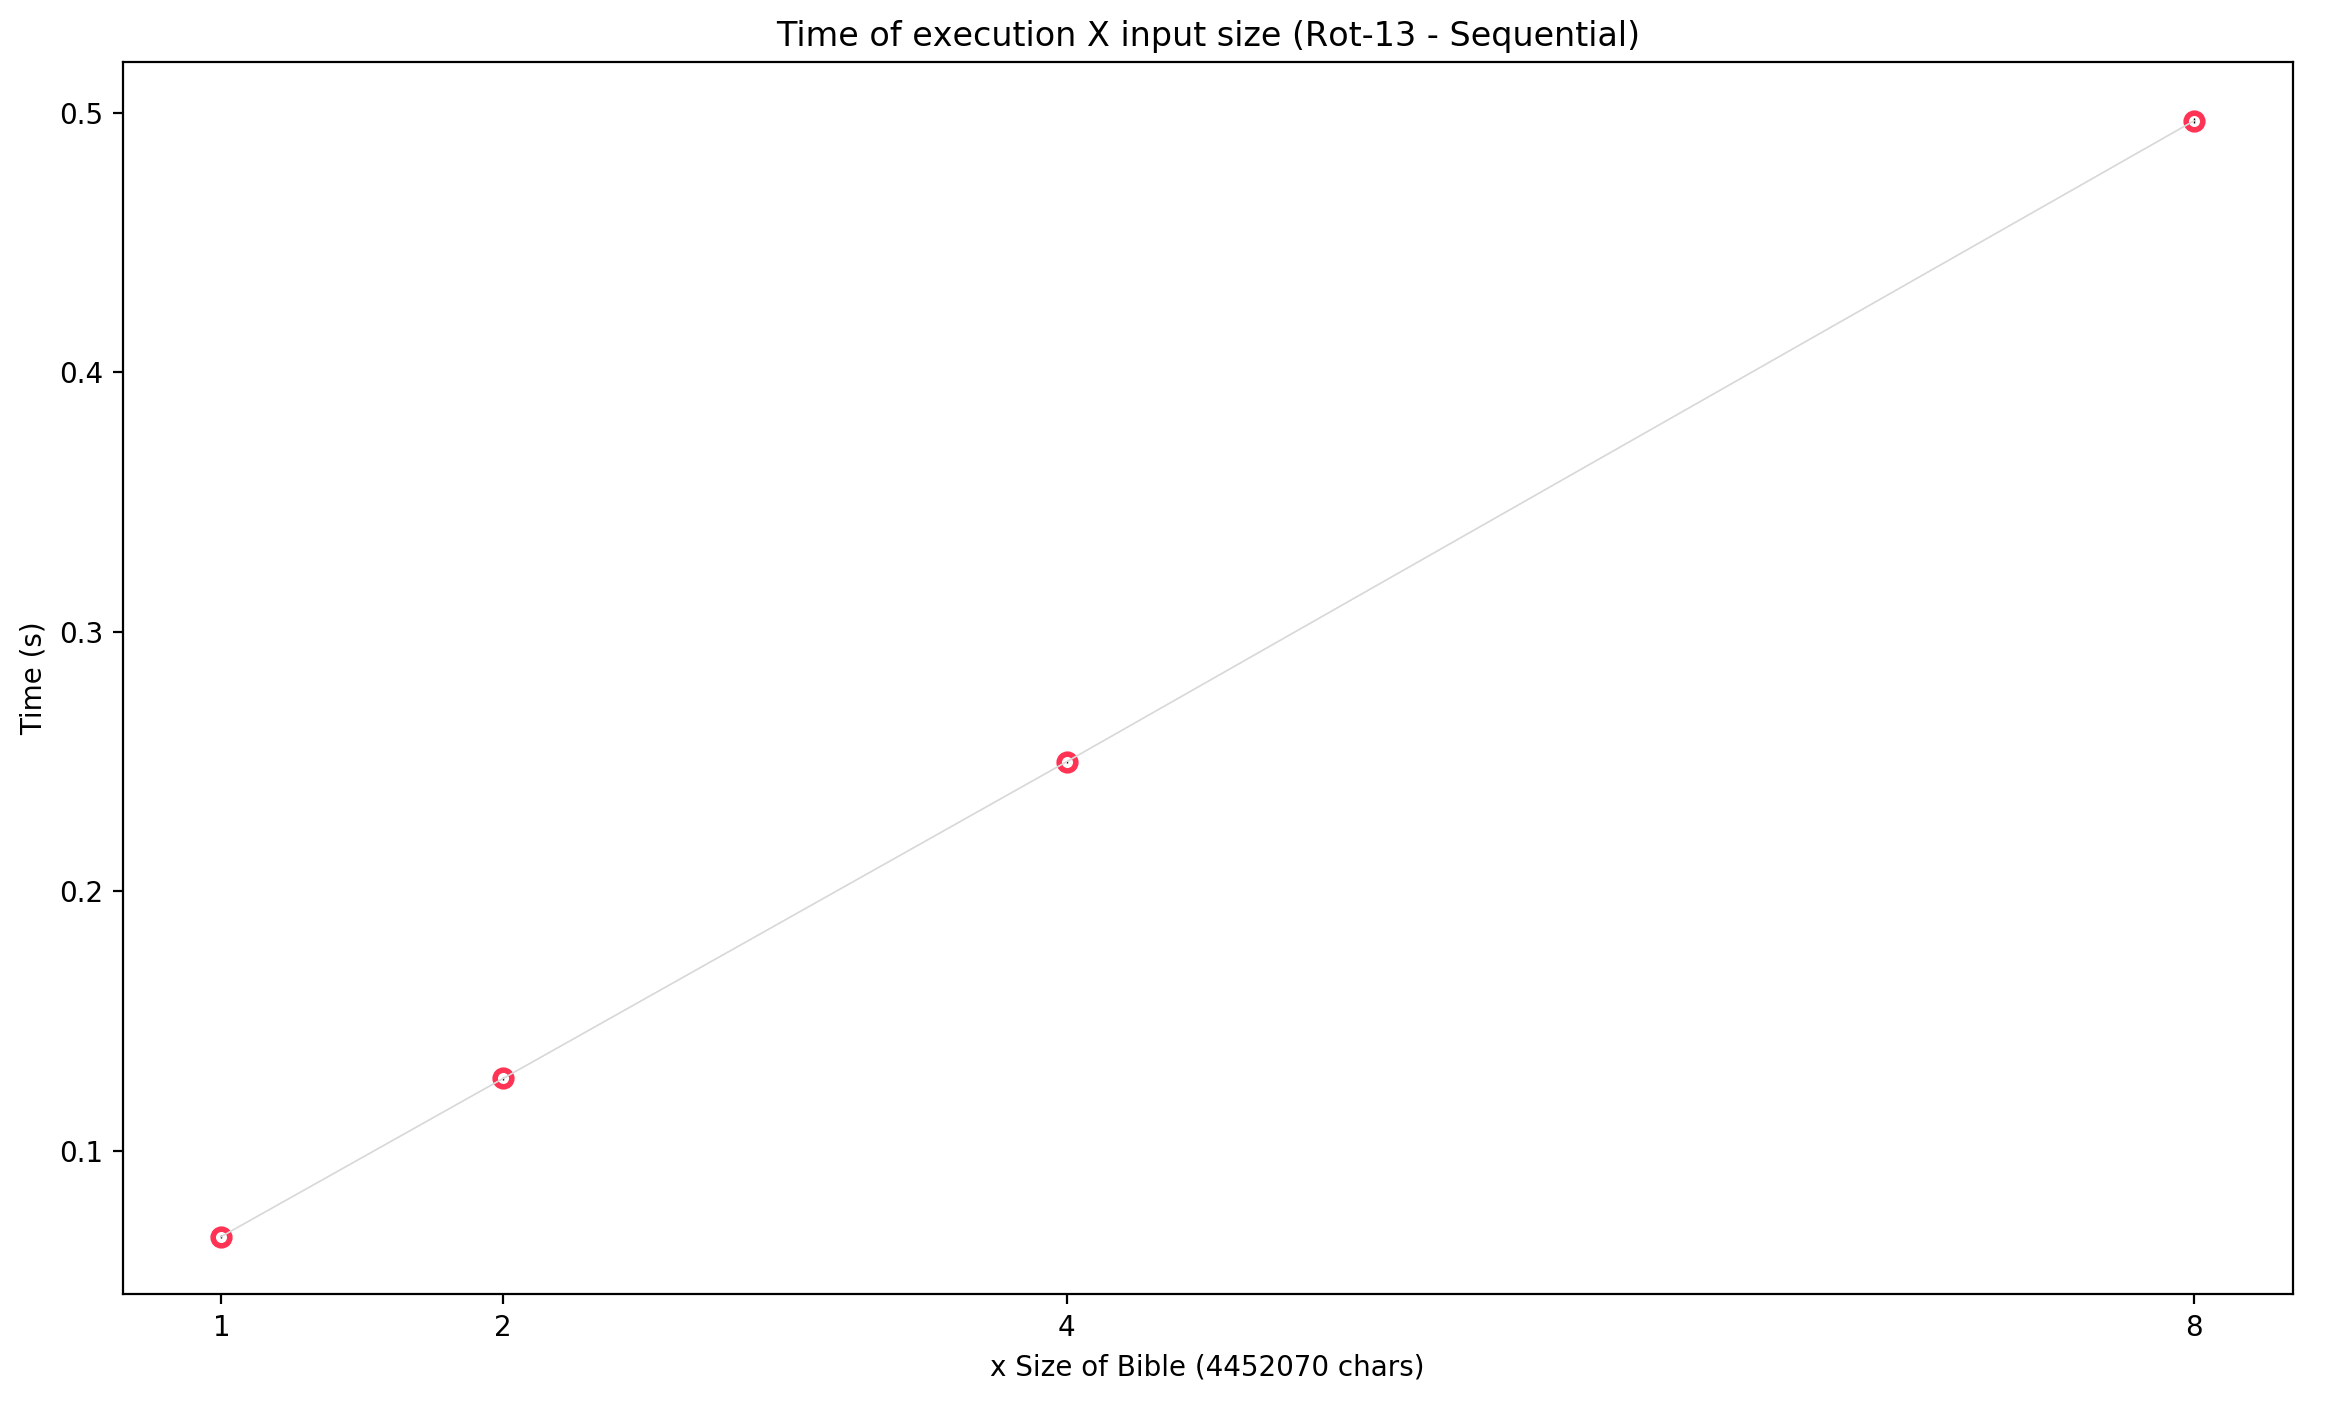
\includegraphics[scale=.65]{img/rot13_seqXpar/timeXsize_Rot-13 - Sequential.png}}
%\end{figure}

Apesar de 8 vezes o tamanho da bíblia (35.616.560 caracteres) ser um
número bastante grande, até mesmo o algoritmo sequencial o realiza em
apenas meio segundo. Esperamos que a implementação paralela, realize os
cálculos pelo menos mais rápido que a implementação sequencial:

%\begin{figure}[H]
    %\makebox[\textwidth][c]{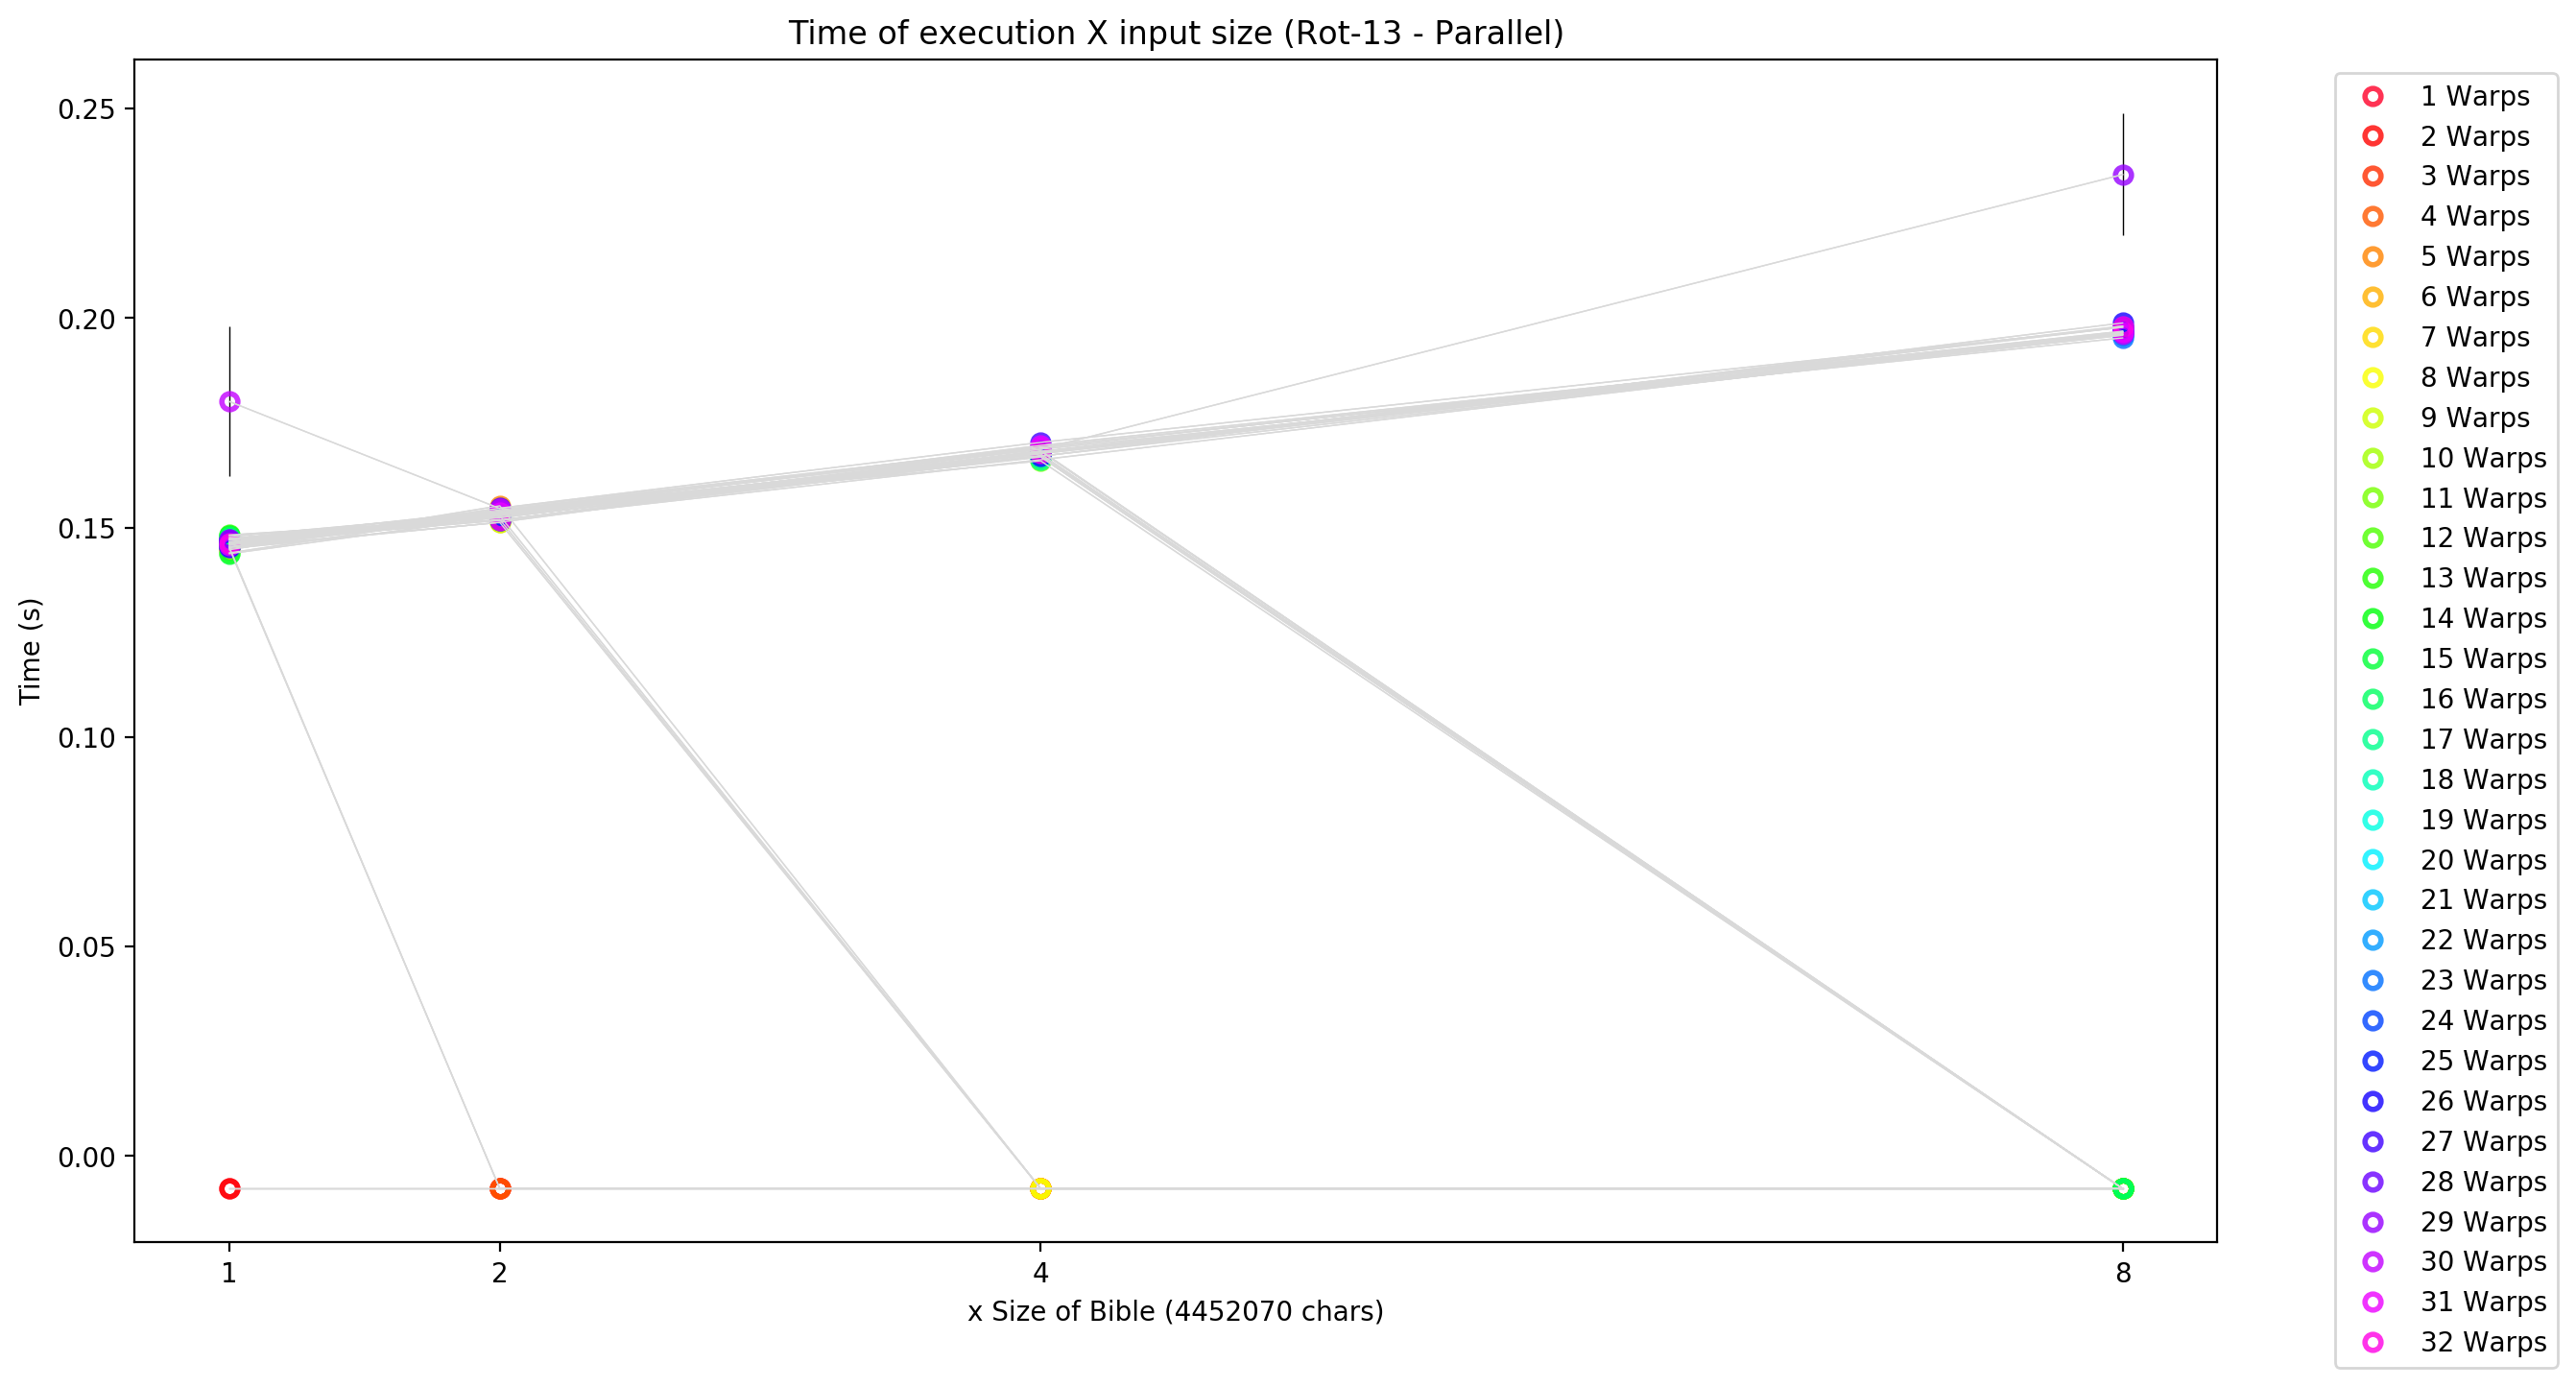
\includegraphics[scale=.55]{img/rot13_seqXpar/timeXsize_Rot-13 - Parallel.png}}
%\end{figure}

Como esse gráfico possui mais informações analisemos-o com mais cuidado.
O eixo Y representa o tempo levado para o algoritmo ser executado.
O eixo X representa o tamanho dos arquivos de entrada. Em cada execução
do programa, utilizamos um valor de threads por bloco. 1 warp 
representa 32 threads. Para cada valor de 1 a 32 warps, uma cor é
utilizada no gráfico. Além disso, para algumas combinações de número de
threads e de tamanho de entrada, há falha ao passar tais argumentos
para a GPU. Nesses casos representamos o tempo do algoritmo por um valor
um pouco abaixo de 0 no gráfico. Comecemos a analisar o gráfico.

Para cores roxas e mais azuladas, notamos que elas seguem o mesmo padrão
linear de aproximadamente 0,15s a 0,18s. Os valores aonde há erro
ocorrem, pois o número de blocos necessários para a combinação
ultrapassaria o número máximo de blocos da GPU. Por exemplo para 1 warp
(32 threads) e tamanho de entrada 1 Bíblia (4.452.070 caracteres) há a
necessidade de 139.128 blocos, que ultrapassa o número máximo de blocos
da GPU (65535). Ou seja, quando aumentamos o tamanho do arquivo de
entrada, algum dos valores de número de warps por bloco passam a ser
inválidos, pois iriam requirir blocos demais. É interessante notar que
para os valores adequados de warps por blocos o tempo de execução do
programa é o mesmo:

%\begin{figure}[H]
    %\makebox[\textwidth][c]{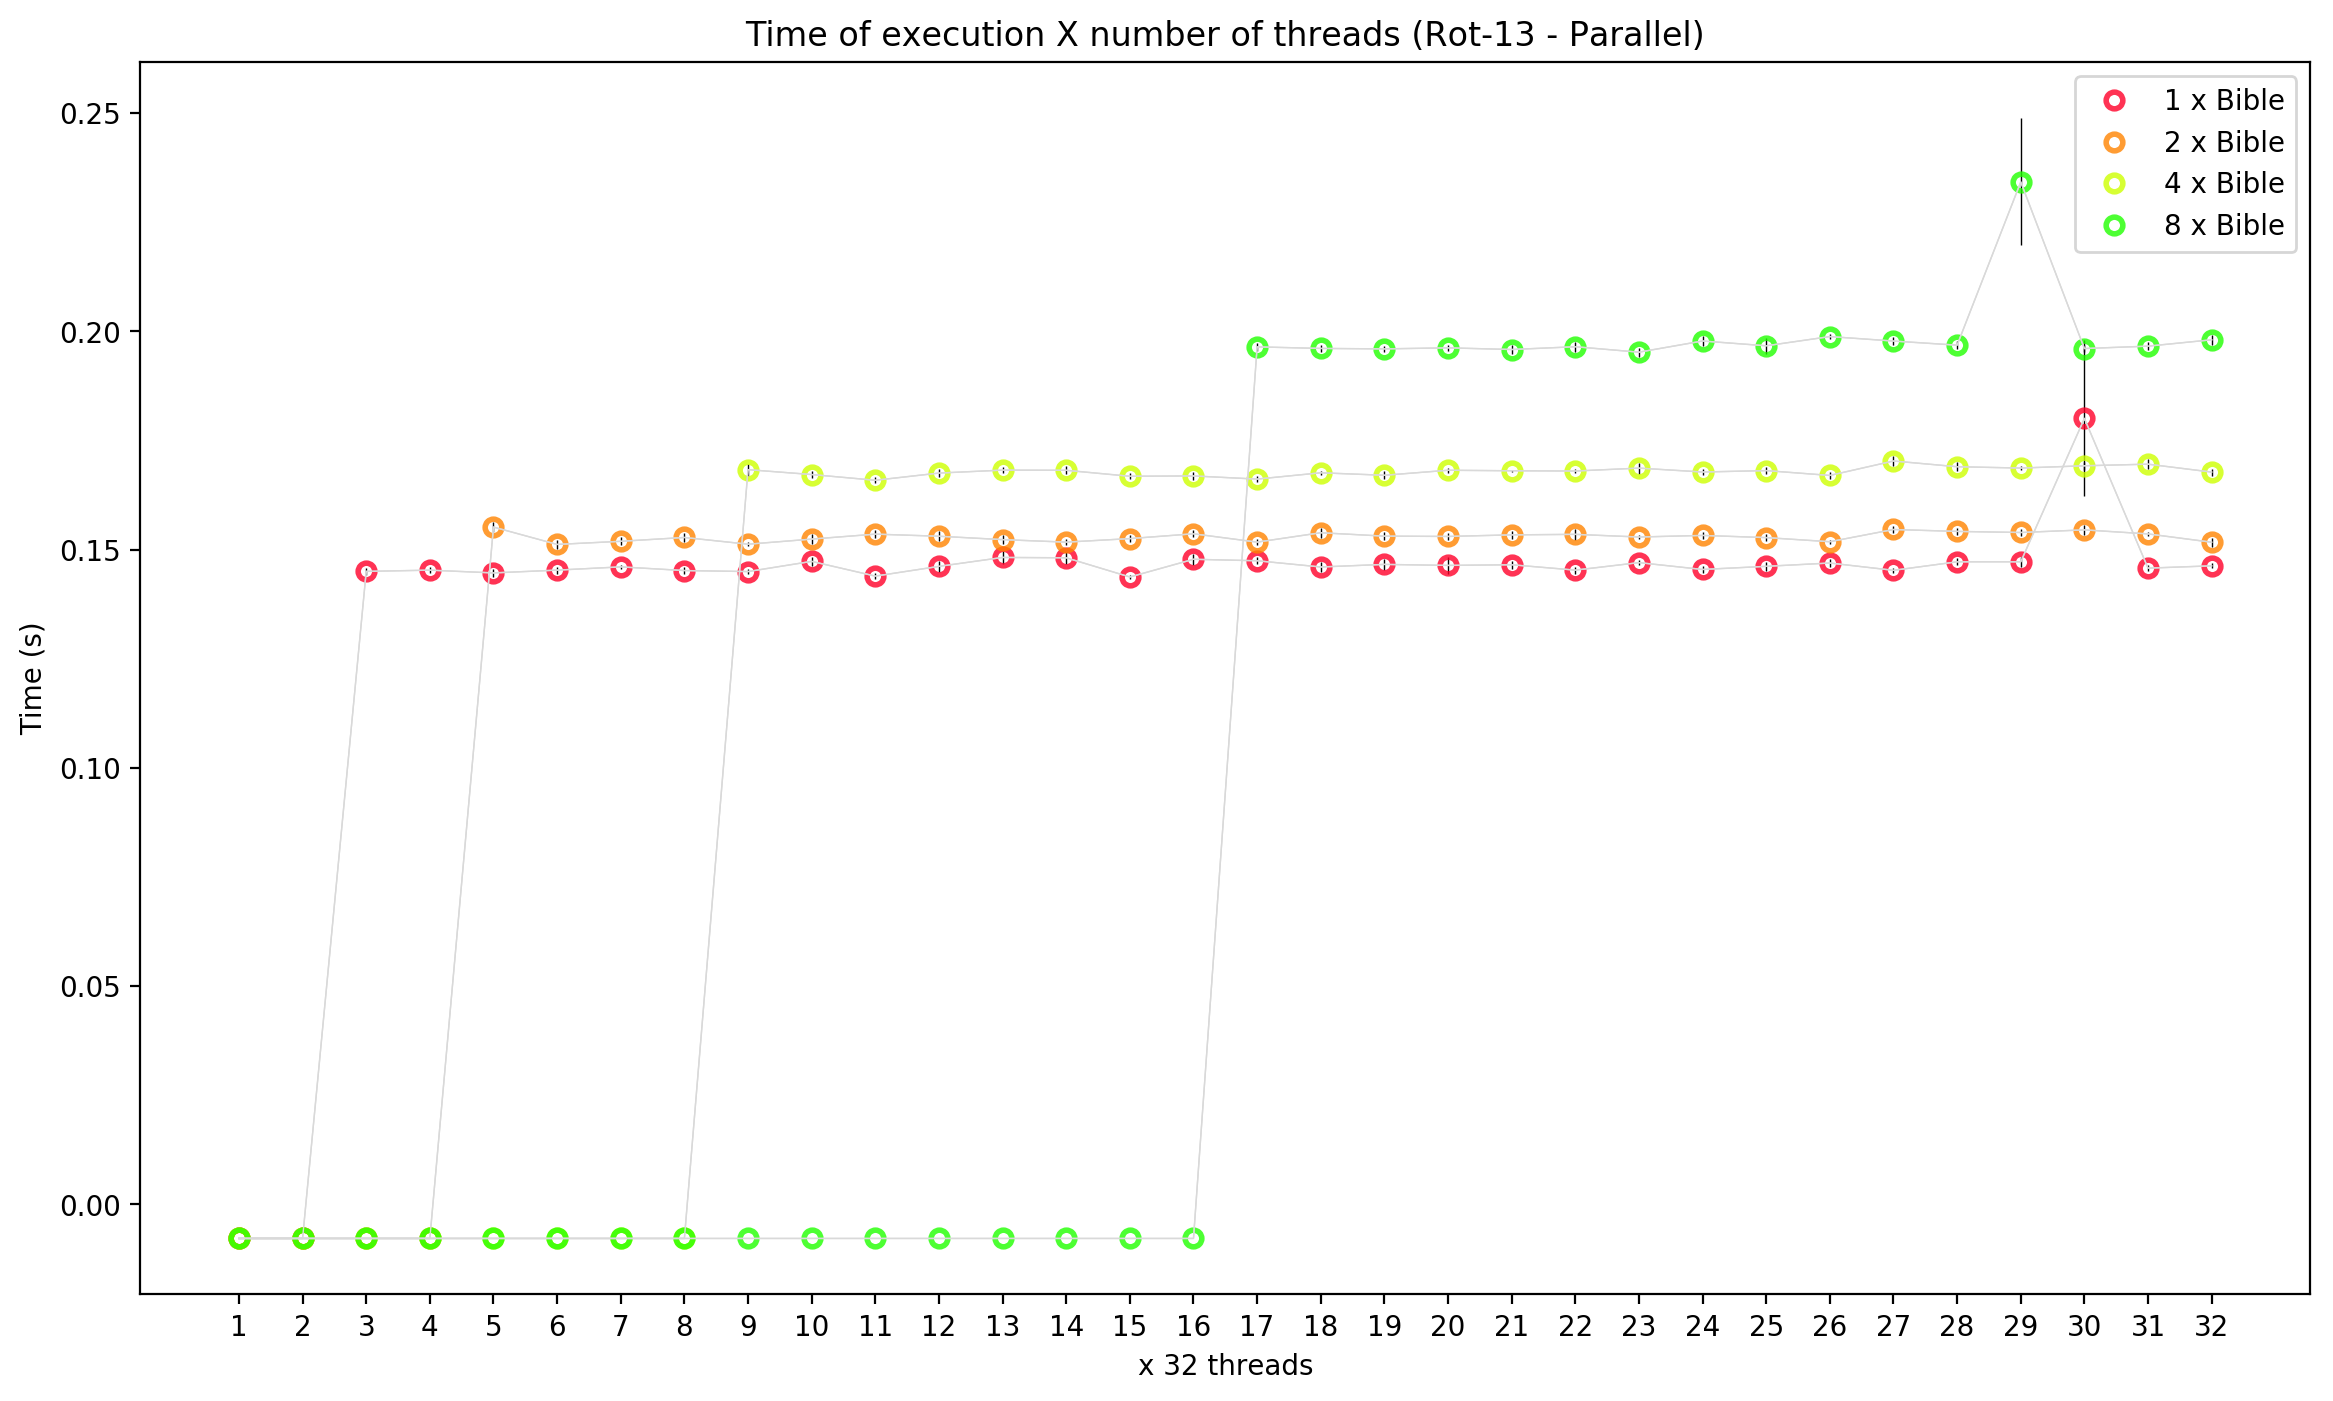
\includegraphics[scale=.55]{img/rot13_seqXpar/timeXthread_Rot-13 - Parallel.png}}
%\end{figure}

Nesse gráfico o eixo Y representa o tempo de execução do programa
enquanto o eixo X representa o número de threads por bloco. Para cada
tamanho de entrada uma cor é dada. Nesse gráfico fica claro como para o
mesmo tamanho de entrada, independente do número de threads por bloco o
tempo para a execução é o mesmo. No entanto o tempo cresce de acordo com
o tamanho da entrada. Esse é um resultado inesperado, pois como os 
valores são processados em paralelo não esperávamos que o tempo fosse
aumentar.

Faremos agora uma comparação entre a implementação sequencial e a paralela:

%\begin{figure}[H]
    %\makebox[\textwidth][c]{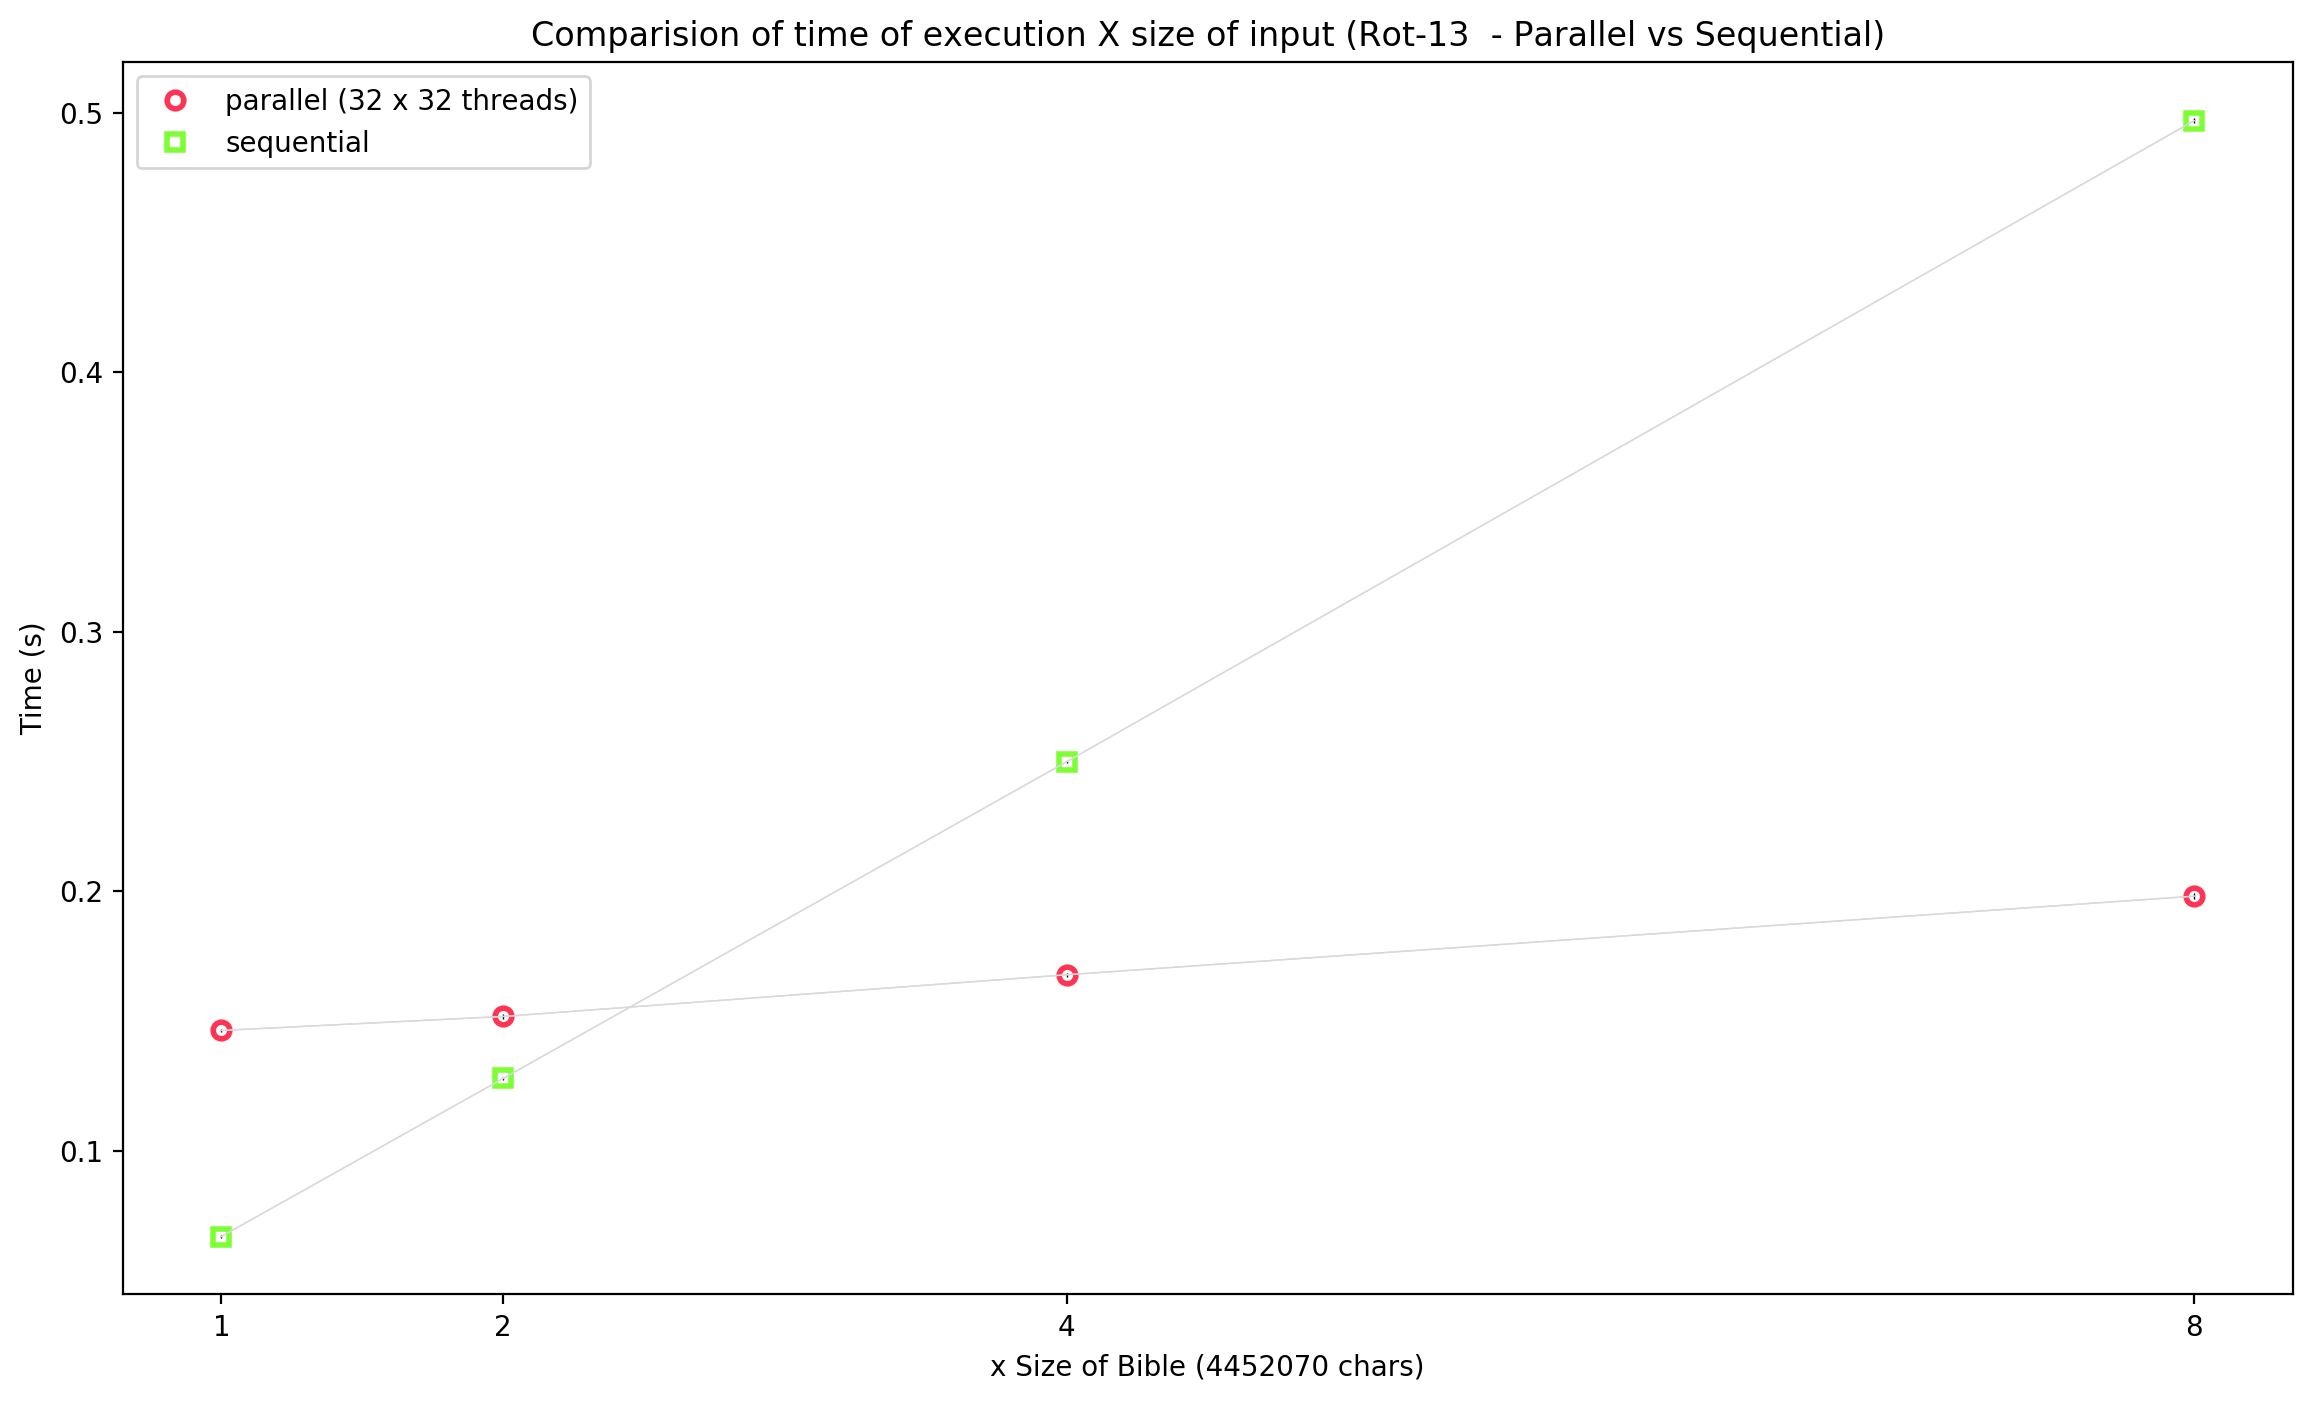
\includegraphics[scale=.55]{img/rot13_seqXpar/compare_timeXsize_Rot-13 - Parallel vs Sequential.png}}
%\end{figure}

Como discutido anteriormente, como o tempo de execução independe do
número de threads por bloco, escolhemos 32 x 32 threads, pois
garantimos que o número de blocos necessários serão validos.

Notamos um comportamento interessante, onde para 1 e 2 vezes a Bíblia,
o algoritmo sequencial é mais rápido que o paralelo. No entanto,
para valores um pouco maior que 2 vezes o tamanho da Bíblia a
implementação paralela é mais rápida. Talvez isso ocorra, devido á
transferência de dados para a GPU, que leva um tempo extra em relação à
implementação sequencial, porém como a os dados são processados
paralelamente, a taxa de crescimento do tempo em relação ao tamanho dos
arquivos de entrada da implementação paralela é menor do que o da
sequencial. De fato, talvez a implementação paralela só cresça devido a
operação de leitura de arquivo que ocorre sequencialmente para ambos os
algoritmos. Comparemos com o seguinte gráfico:

%\begin{figure}[H]
    %\makebox[\textwidth][c]{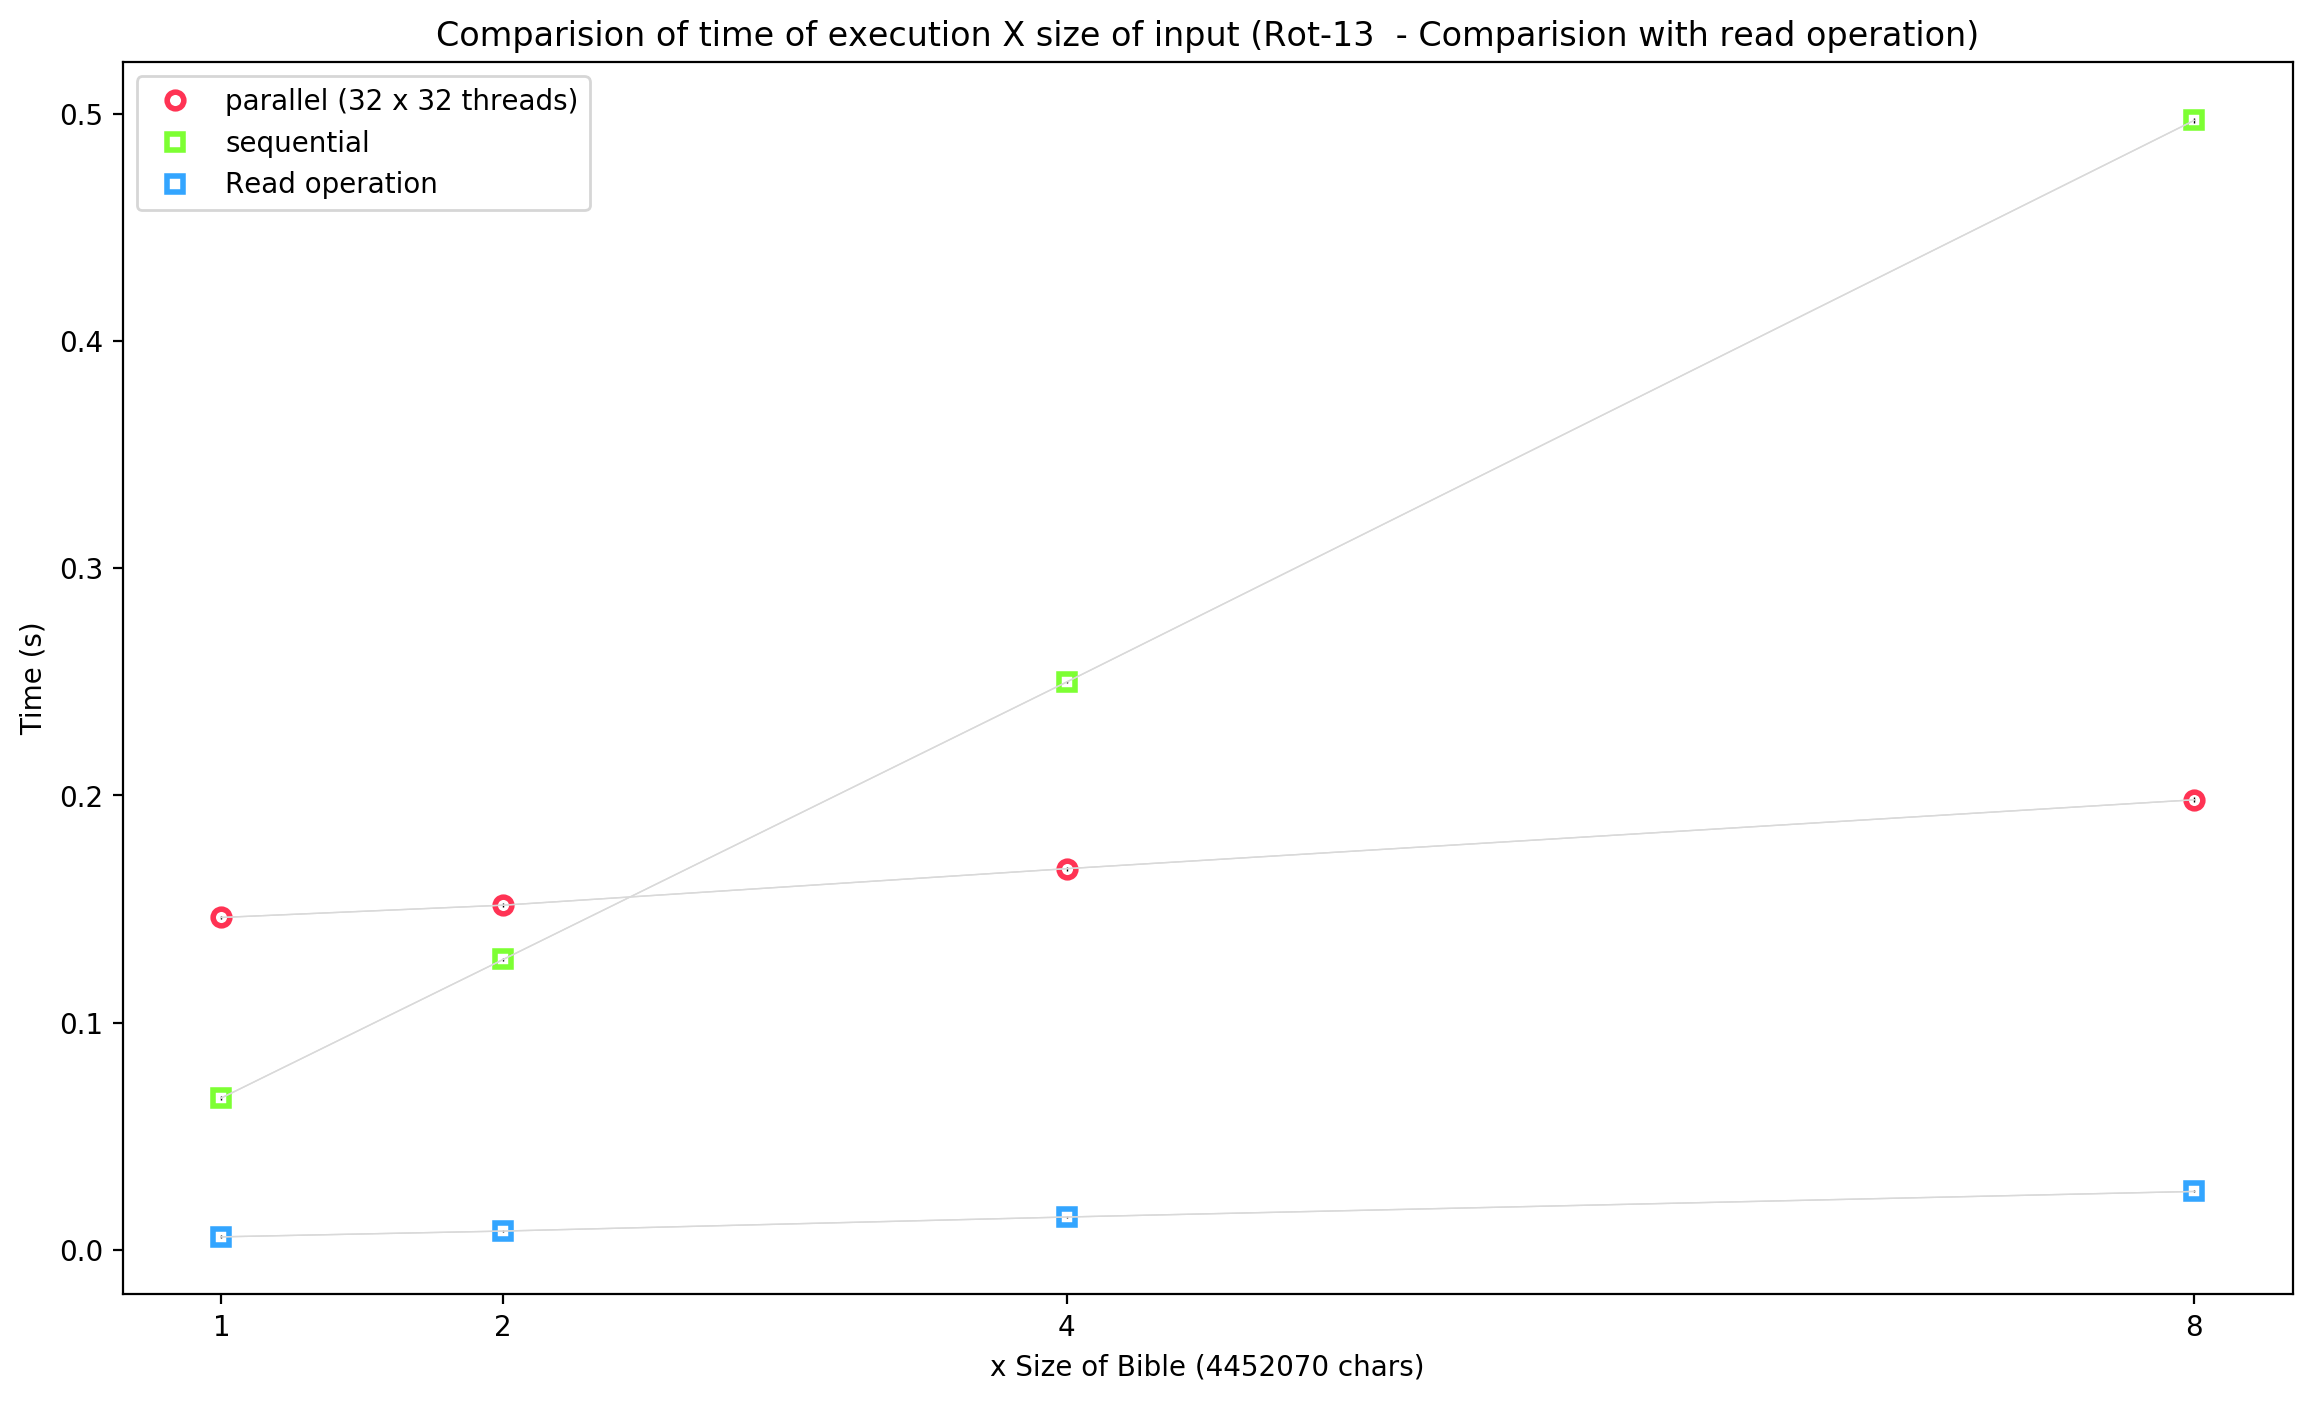
\includegraphics[scale=.55]{img/rot13_seqXpar/compare_read_Rot-13 - Comparision with read operation.png}}
%\end{figure}

Para gerar os dados dos pontos azuis, executamos um programa que somente
lê um arquivo e o guarda em um vetor de caracteres. Essa é a mesma
função utilizada nas duas implementações do algoritmo rot13. 

Nota-se que a inclinação do tempo de leitura é bastante similar com a da
implementação paralela. Portanto se pudéssemos retirar a leitura do 
algoritmo paralelo, o tempo para encriptação seria o mesmo independente
do tamanho de entrada. É claro que isso se limita aos valores máximos
de threads por bloco e de blocos por GPU. 

\subsection{Vigenere}


%%%%%%%%%%%%%%%%%%%%% CONCLUSAO %%%%%%%%%%%%%%%%%%%%%%%%%%%%%%%%%%%%%%%%
\newpage
\section{Conclusão}

\end{document}
